\PassOptionsToPackage{unicode=true}{hyperref} % options for packages loaded elsewhere
\PassOptionsToPackage{hyphens}{url}
%
\documentclass[]{article}
\usepackage{lmodern}
\usepackage{amssymb,amsmath}
\usepackage{ifxetex,ifluatex}
\usepackage{fixltx2e} % provides \textsubscript
\ifnum 0\ifxetex 1\fi\ifluatex 1\fi=0 % if pdftex
  \usepackage[T1]{fontenc}
  \usepackage[utf8]{inputenc}
  \usepackage{textcomp} % provides euro and other symbols
\else % if luatex or xelatex
  \usepackage{unicode-math}
  \defaultfontfeatures{Ligatures=TeX,Scale=MatchLowercase}
\fi
% use upquote if available, for straight quotes in verbatim environments
\IfFileExists{upquote.sty}{\usepackage{upquote}}{}
% use microtype if available
\IfFileExists{microtype.sty}{%
\usepackage[]{microtype}
\UseMicrotypeSet[protrusion]{basicmath} % disable protrusion for tt fonts
}{}
\IfFileExists{parskip.sty}{%
\usepackage{parskip}
}{% else
\setlength{\parindent}{0pt}
\setlength{\parskip}{6pt plus 2pt minus 1pt}
}
\usepackage{hyperref}
\hypersetup{
            pdftitle={Target-based site prioritization under climate change using quadratic network flow},
            pdfauthor={Derek Corcoran},
            pdfborder={0 0 0},
            breaklinks=true}
\urlstyle{same}  % don't use monospace font for urls
\usepackage[margin=1in]{geometry}
\usepackage{longtable,booktabs}
% Fix footnotes in tables (requires footnote package)
\IfFileExists{footnote.sty}{\usepackage{footnote}\makesavenoteenv{longtable}}{}
\usepackage{graphicx,grffile}
\makeatletter
\def\maxwidth{\ifdim\Gin@nat@width>\linewidth\linewidth\else\Gin@nat@width\fi}
\def\maxheight{\ifdim\Gin@nat@height>\textheight\textheight\else\Gin@nat@height\fi}
\makeatother
% Scale images if necessary, so that they will not overflow the page
% margins by default, and it is still possible to overwrite the defaults
% using explicit options in \includegraphics[width, height, ...]{}
\setkeys{Gin}{width=\maxwidth,height=\maxheight,keepaspectratio}
\setlength{\emergencystretch}{3em}  % prevent overfull lines
\providecommand{\tightlist}{%
  \setlength{\itemsep}{0pt}\setlength{\parskip}{0pt}}
\setcounter{secnumdepth}{5}
% Redefines (sub)paragraphs to behave more like sections
\ifx\paragraph\undefined\else
\let\oldparagraph\paragraph
\renewcommand{\paragraph}[1]{\oldparagraph{#1}\mbox{}}
\fi
\ifx\subparagraph\undefined\else
\let\oldsubparagraph\subparagraph
\renewcommand{\subparagraph}[1]{\oldsubparagraph{#1}\mbox{}}
\fi

% set default figure placement to htbp
\makeatletter
\def\fps@figure{htbp}
\makeatother

\usepackage{booktabs}
\usepackage{longtable}
\usepackage{array}
\usepackage{multirow}
\usepackage{wrapfig}
\usepackage{float}
\usepackage{colortbl}
\usepackage{pdflscape}
\usepackage{tabu}
\usepackage{threeparttable}
\usepackage{threeparttablex}
\usepackage[normalem]{ulem}
\usepackage{makecell}
\usepackage{xcolor}

\title{Target-based site prioritization under climate change using quadratic network flow}
\author{Derek Corcoran}
\date{}

\begin{document}
\maketitle

\hypertarget{introduction}{%
\section{Introduction}\label{introduction}}

Currently, 14.9\% of terrestrial area is a part of the global protected area network (UNEP-WCMC 2018). However, most protected areas have not been created using prioritization tools developed to maximize outcomes such as species or ecosystems conservation based on current biodiversity patterns, resulting in under performing conservation networks globally (Rodrigues et al. 2004; Jenkins et al. 2015). The situation could be even worst when we take into account that species distributions are expected to change over time as a result of anthropogenic climate change (Araújo et al. 2004; Chen et al. 2011; Lenoir et al. 2008; Regos et al. 2016) if species that are now protected migrate out of protected areas in the future (Marquet, Lessman, and Shaw 2019; Alagador, Cerdeira, and Araújo 2014; Hannah et al. 2007; Araújo et al. 2004).

Different approaches and workflows have been recently developed with the aim to inform conservation planning in adapting conservation networks to climate change (Marquet, Lessman, and Shaw 2019). One of the main avenues of research focuses on finding areas that are able to include both species current and future projected distributions. However, a review by Jones et al. (2016) showed that more than 90\% of the prioritization planning studies following this approach did only consider biodiversity needs in two time steps: where does biodiversity occur under current climatic conditions and where is it projected to occur at a certain year ahead in the future (typically, at the end of the century). The concern is that these solutions may be insufficient to effectively allow species meet their future suitable ranges from their current distributions, or that solutions are not adequately optimized. A major problem preventing more adequate solutions is methodological limitation. Currently, the most used tools for conservation planning are Marxan, Prioritizr and Zonation (Di Minin et al. 2014; Hanson et al. 2019). From these, Zonation includes more advanced options to prioritize conservation under climate change scenarios, as conservation features may be explicitly linked through interaction (i.e.: Reside, VanDerWal, and Moran (2017)). This allows for simultaneous prioritization of a species current range, its modeled future range, and the connectivity between the two limited by a species' capacity to disperse, but it is restricted to using one future modeled range per species. On the other hand, Prioritizr and Marxan do not include specific options to consider climate change related biodiversity needs.

\begin{table}[H]
\centering
\begin{tabular}{lllll}
\toprule
 & Network flow & Zonation & Migclim & Prioritizr\\
\midrule
Considers more than 2 time-slices & Yes & No & Yes & No\\
Can add species to the solutions afterwards & Yes & No & Yes & No\\
Keep track of species dispersal routes & Yes & Yes & Yes & No\\
Solves for conservation targets & Yes & Yes & No & Yes\\
Considers cost as part of the solution & Yes & Yes & No & Yes\\
\bottomrule
\end{tabular}
\end{table}

In order for the species to move from areas were they are currently protected to the future protected areas, their route has to be protected as well, that is the biological corridors that they will use (Nuñez et al. 2013; Rosenberg, Noon, and Meslow 1997). In this particular case, these routes might be referred as climatic biological corridors. The planning and creation of these biological corridors correspond to adaptive measures to environmental changes that would mitigate the impacts of the climate crisis (Hannah et al. 2007). In that context, climate biological corridors should consider the progressivity of the effects of the climate crisis, including changes in suitable climatic conditions and in land use and habitat fragmentation, in order to evaluate the feasibility of the species reaching their future available habitat.

There have been several approaches trying to model biological corridors. Local approaches have focus just in one or a few species (Alagador, Cerdeira, and Araújo 2014; Cushman et al. 2013; Gregory et al. 2014) or group of species (Beier, Majka, and Bayless 2007; Phillips et al. 2008; Williams et al. 2005), not being able to be use for planning for lack of species or be in confined spaces, respectively. A continental approach was made by Lawler et al. (2013), who modeled biological corridors in the Americas. Even when that model was made for close to 3,000 species, it did not consider species dispersal speed, and it did not use the information on species migration routes to identify priority areas that are climatically resilient. However, among these articles, the work of Phillips et al. (2008) incorporates the use of the Network Flow optimization method (Ahuja, Magnanti, and Orlin 1993) in order to solve the problem expressed by Williams et al. (2005), generating a solution 33\% more efficient than previous optimization methods. This makes this methodology one of the most promising ways of solving conservation planning problems through the use of biological corridors.

In its traditional use, Network Flow gives the best possible solution given constrains (Phillips et al. 2008). If we looked at the solution for a species in a raster, every cell would have a value of either one or zero, where one would be a cell necessary for the conservation of the species or a zero if it is not necessary. This best solution, however, only represents one of the possible solutions to conserve a species, and does not give us any alternatives.

Considering there is a trade-off between efficiency and resilience in systematic conservation planning (Fischer et al. 2009), and even when Linear Cost Network Flow is the most efficient solution in terms of area needed for the conservation of biological corridors, it will show us only one possible option of several, we present Quadratic Cost Network Flow as alternative solution for conservation planning that is more rescilient than Linear Cost Network Flow, while still being a very efficient method.

With Quadratic Network Flow, where for every species we would still get a value of one if the cell is irreplaceable for the solution, zero if that cell is not needed, and an intermediate value for cells that are one of many alternative solutions for a given species, this is, for every cell we have an irreplaceability index. Spatial planning is a complex endeavor where agendas and/or needs evolve rapidly and several alternative sub-optimal solutions might be needed in order to navigate this complex decisions. Quadratic Cost Network Flow fills that gap by 1. Identifying irreplaceable cells, that if not taken into consideration species would become extinct, and 2.- Creating a buffer around the most efficient solutions that gives us alternatives on the event the mos efficient solution is not feasible.

The aim of this article is to present a new method of working with network flow on conservation planning using quadratic costs, while at the same time comparing its results and implications with Linear Cost Network Flow,first using a toy model followd by a proof of concept, using the Northern Tropical Andes ecorregion as an example.

\hypertarget{methods}{%
\section{Methods}\label{methods}}

In order to show an easy example on how Network Flow works for one species, we will use an hypothetical species that inhabits an hypothetical linear environment composed by 7 cells. In figure \ref{fig:Phil} we can see the projection of the potential distribution of this species in 2 different times (\(T_0\) and \(T_1\)). In in \(T_0\), there are 4 different cells that are suitable for the species: cells 2, 5, 6 and 7. For \(T_1\) there are 5 cells that are suitable for the species: cells 1, 2, 3, 4 and 7. The problem we want to solve is that we want to preserve a target amount of space for every time-slice, which will have two constraints, 1.- the species has a dispersal limitation. So lets say for example that in the time that goes from \(T_1\) to \(T_0\) our hypothetical species can only move up to one cell, that is, individuals that are present in cell 2 during \(T_0\) could only reach cells 1,2 and 3, but not cells 4 and 7, as seen in figure \ref{fig:PhilNet}. 2.- There wont be any ``amount'' of species gained or lost when individuals move to another time-slice. That is, if a unit of our species flows out from cell 2 in \(T_0\) there can't be a unit of that species in cell 2, and another in cell 3 in \(T_1\), that is there is a conservation of flow between times.

\begin{figure}
\centering
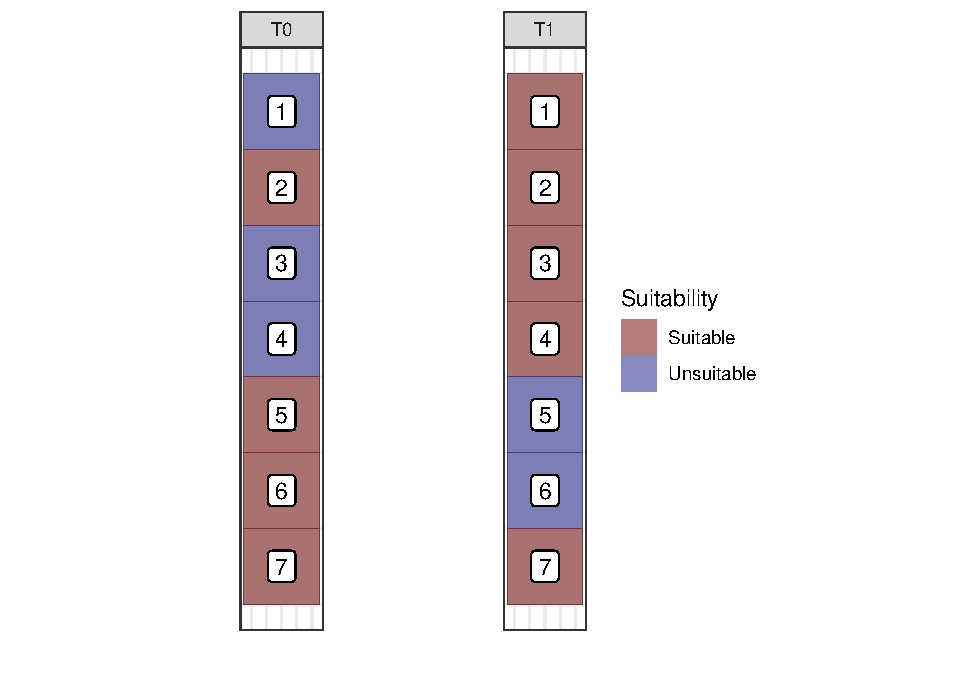
\includegraphics{TagetBasedNew_files/figure-latex/Phil-1.pdf}
\caption{\label{fig:Phil}Hypothetical potential distribution of a species over two timeslices}
\end{figure}

\begin{figure}
\centering
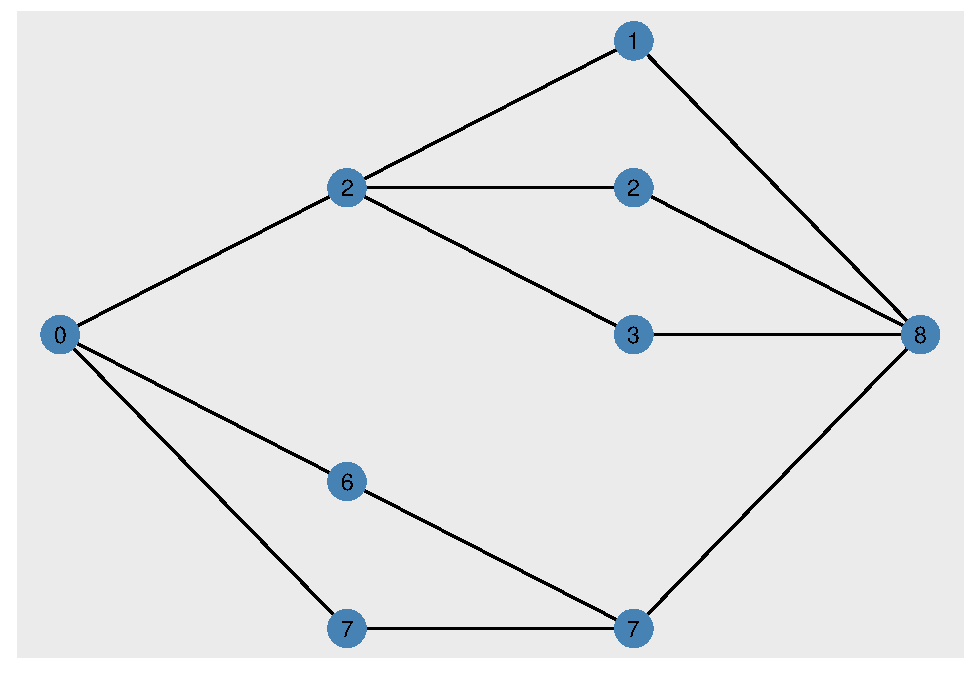
\includegraphics{TagetBasedNew_files/figure-latex/PhilNet-1.pdf}
\caption{\label{fig:PhilNet}Network created from the Species Distribution models taking into account dispersal distance}
\end{figure}

Those are the constraints of the optimization and the objective of the optimization is to minimize the cost. In order to be able to do that, we need a cost layer and in this case we will use the layer shown in figure \ref{fig:PhilCost}. The cells with a value of zero here represent protected areas (cell 1 and 3), while the black cells represent unavailable cells do to the presence of some obstacle such as cities, glaciers, or any other obstacle we want to take out of the possible solutions (cells 4 and 5), all other cells have a value where the most expensive cell (cell 2) has a cost of being incorporated to the network of protected areas of 0.5 while cells 6 and 7 have a lower value (0.25). This costs could be anything from the direct purchase of the area to transform it to a protected area, to the potential conflict with human population.

\begin{figure}
\centering
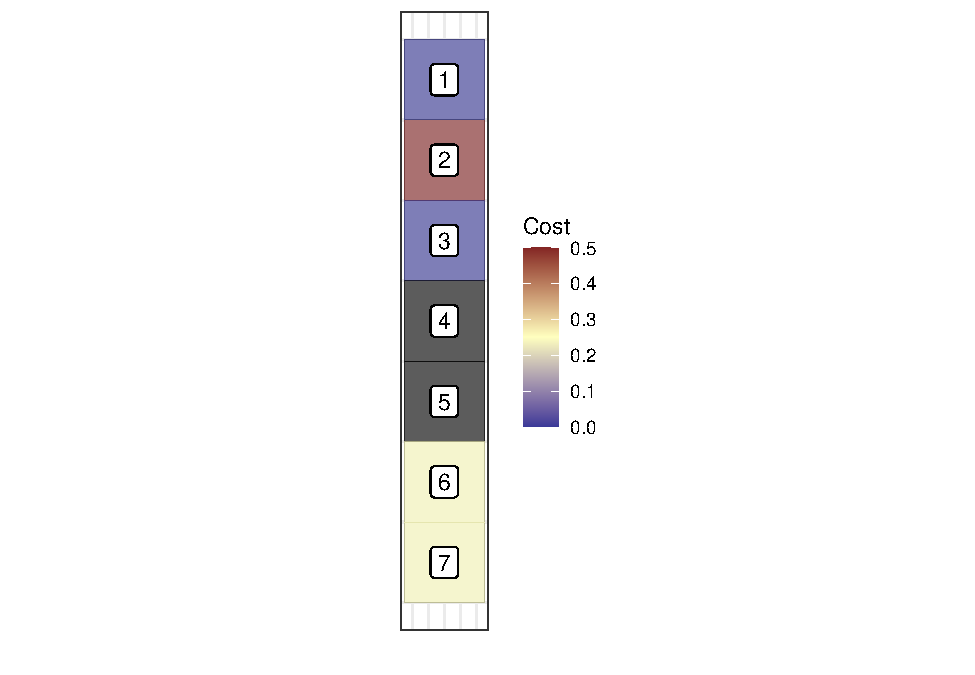
\includegraphics{TagetBasedNew_files/figure-latex/PhilCost-1.pdf}
\caption{\label{fig:PhilCost}Cost layer for the problem the cells with a value of zero represent a protected area, while the black cells represent unavailable cells do to the presence of some obstacle such as cities}
\end{figure}

\hypertarget{stating-the-problem}{%
\subsection{Stating the problem}\label{stating-the-problem}}

Let's assume that we want to preserve the species in figure \ref{fig:Phil}, and that we know that we need at least two cells of area for the species in each time-slice (hereafter number of chains). We know that the species can only move 111 kilometers in the time that passes from one time slice to another (that is one cell) and we want the solution to be the least expensive taking into account the cost layer.

\hypertarget{methods-northern-tropical-andes}{%
\subsection{Methods Northern Tropical Andes}\label{methods-northern-tropical-andes}}

\begin{figure}

{\centering 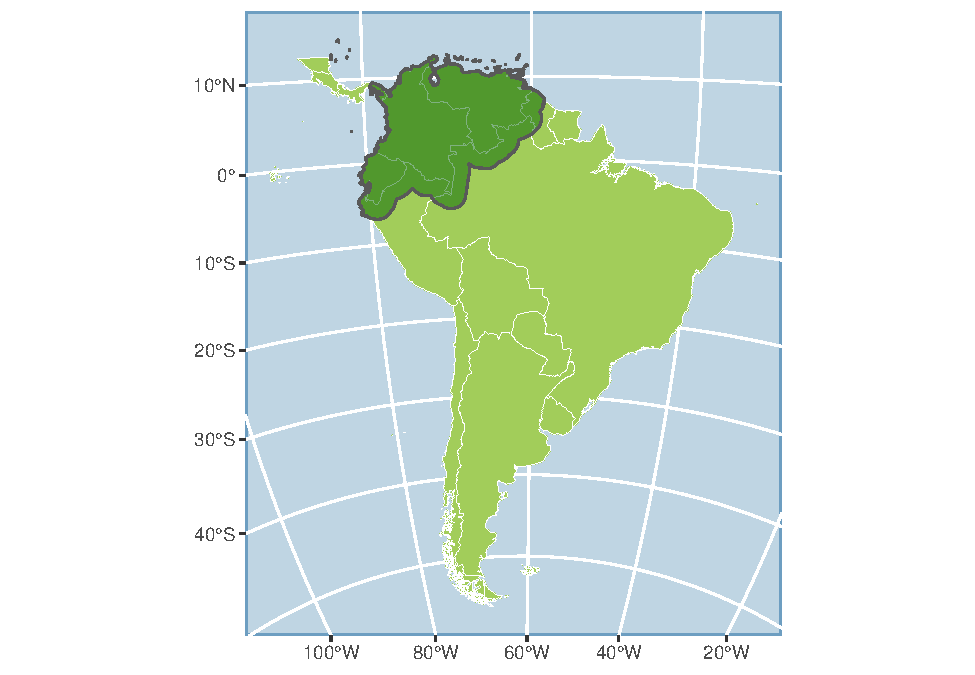
\includegraphics{TagetBasedNew_files/figure-latex/MapArea-1} 

}

\caption{Map of Southamerica, the darkened area is the area where the priorization was performed}\label{fig:MapArea}
\end{figure}

The studied area was the Northern Tropical Andes, including the countries of Colombia, Venezuela and Ecuador (Figure \ref{fig:MapArea}). To avoid pixels on countries' borders receiving a lower priority due to a boundary effect, we extended the analyses to a buffer of 200 kilometers around their terrestrial domains. The study area encompasses a total of 3,632,762 square kilometres.

\hypertarget{global-circulation-models}{%
\subsection{Global circulation models}\label{global-circulation-models}}

Global Circulation Models (GCMs) are predictive models that use fluid models\ldots{}
In this study, four GCM models were selected to project species distribution using the GCMcompareR shiny app (Fajardo et al. 2020), we followed the story-lines approach (Zappa and Shepherd 2017) and selected a GCM warmer and wetter, warmer and dryer, colder and wetter, and colder and dryer than the ensemble. The selected models where cc, cn, la, mp.

\hypertarget{species-selection}{%
\subsection{Species selection}\label{species-selection}}

We used a set of 671 species of plants and vertebrates to conduct the analyses(see Table S1 for the full list of species). We only restricted the analysis to species that are endemic to the three studied countries with the purpose to consider all possible solutions for each analysed organism. For each species, we collected and curated a database of occurrences, and built species distribution models to project species potential distributions and forecast environmental suitability under two climate change scenarios.
.

For plants, all presences were collected from the BIEN database. The BIEN database is a product of a workflow of several tools, including two softwares: Taxonomic Name Resolution Service (Boyle et al. 2013) and Geographic Name Resolution Service (Boyle 2019). The first resolves and corrects sinonymous taxa. The second validates, eliminates or flags coordinates accordingly. In this research, only records where the scientific name was clear to the species level, passed all geographic validations, was certain to be a native species, and was not part of a plot were included.

Vertebrates ocurrences were extracted form GBIF, Vertnet, and Global Restricted range bird species data bases. We only used presences from 1950 onwards, that were recorded by human observation. All centroids and longitudes or latitudes of exactly zero were removed. Points were also removed if they were further than 500 Km from the ranges developed by IUCN.

\hypertarget{species-distribution-models.}{%
\subsection{Species Distribution Models.}\label{species-distribution-models.}}

The Dismo Package (Hijmans et al. 2017) was used to generate Species Distribution Models with the Maxent algorithm (Phillips, Anderson, and Schapire 2006; Merow, Smith, and Silander Jr 2013). We used the methods described in Merow, Smith, and Silander Jr (2013) and Merow et al. (2014) to generate models with less overfitting and with less complex responses to variables. Modeling domains were limited to a spatial buffer of 500km within any geovalid occurrence record. Background sampling consisted in a random sample of 50,000 points. Five model replicates were used in fitting the model, and the average was used as the final species model. 30\% of occurrence records were reserved to assess model performance.

Environmental predictor variables were extracted from Worldclim. The 19 bioclimatic variables were checked for colinearity. If two variables were hightly correlated (over xx\% ), the simpler variable was always selected. Variables that considered precipitation only or temperature only, were always chosen over variables that combined both. When variables average over time, the shortest time where always prefered over longer time periods (e.g.~Minimum temperature of the coldest month would be chosen over minimum temperature of the coldest quarter). The selected layers were: Mean annual temperature (BIO1), mean diurnal temperature range (BIO2), seasonality of temperature (BIO4), Minimum temperature of the coldest month (BIO6), mean annual precipitation (BIO12), and seasonality of precipitation (BIO15).

An accumulated aridity index was used in an attempt to consider water defficit and dry season length. To calculate this index, we first find the longest stretch of months where potential evapotranspiration is larger than precipitation. Then, we sum the substraction of precipitation and potential evapotranspiration over this period of time.

Additionaly, five soil variables from Soilgrids (De Sousa et al. 2018) were used (depth to bedrock, pH, clay proportion, silt proportion, and bulk density). If one of the variables had multiple strata, we only used the average of the first meter.

\hypertarget{cost-layer}{%
\subsection{Cost layer}\label{cost-layer}}

We used a 2.5 minutes downscaled version of Naidoo and Iwamura (2007) layer of costs in order to estimate the cost per hectare for each area. To generate a cost layer to use for all prioritization algoritms, we modified that layer using the World Database on Protected Areas (WDPA) (UNEP-WCMC 2018) and land-cover (Tuanmu and Jetz 2014): if a cell of the cost layer was inside a proteced area, this was multiplied by zero; if it was outside of a protected area, it was multiplied by one. We only considered protected areas of classes I and II of (WDPA). By doing this, we were able to consider with a cost of zero those areas that are already in the global network of protected areas. Furthermore, every cell that had over 50\% of urbanization or agriculture according to Tuanmu and Jetz (2014) was taken out of the possible solutions. Our aim with this was to exclude areas that are heavily urbanized or intesely used for agriculture and might not be suitable for protection.

\hypertarget{results}{%
\section{Results}\label{results}}

\hypertarget{linear-solution}{%
\subsection{Linear Solution}\label{linear-solution}}

The solution of this problem with Linear Network flow is shown time-slice by time-slice in figure \ref{fig:FinalStack}, and as a final solution in figure \ref{fig:FinalSolution}, which is a raster with all the cells needed to preserve the species. As we can see the flow goes from cell 7 in \(T_0\) to \(T_1\) figure \ref{fig:LinearGraphNEt}, as it is cheaper to stay in the same cell than going to another cell , in this case both cells have a cost of 0.25. In the upper part of the problem, the flow will go from cell 2, to cell 1, this is because the algorithm will always prioritize current protected areas (i.e.~Cells with a cost of 0) over any other cell. This is the most efficient way of solving this problem, but it is not the only way of solving it, in this case it is not even the only way of minimizing the cost. Since the cost of cells 1 and 3 are Zero, the cost would be the same if the flow went from 2 in \(T_0\) to either 1, or 3 in \(T_1\), or even the decision was to stay in cell 2, because even when the cost of cell 2 is higher than in cell 1 or 3, it is already chosen as part of the solution and it wouldn't add to the cost to choose it again for \(T_2\). This is where Quadratic Network Flow is useful, since it recognices different alternatives and with it it gives us more reciliency.

\begin{figure}
\centering
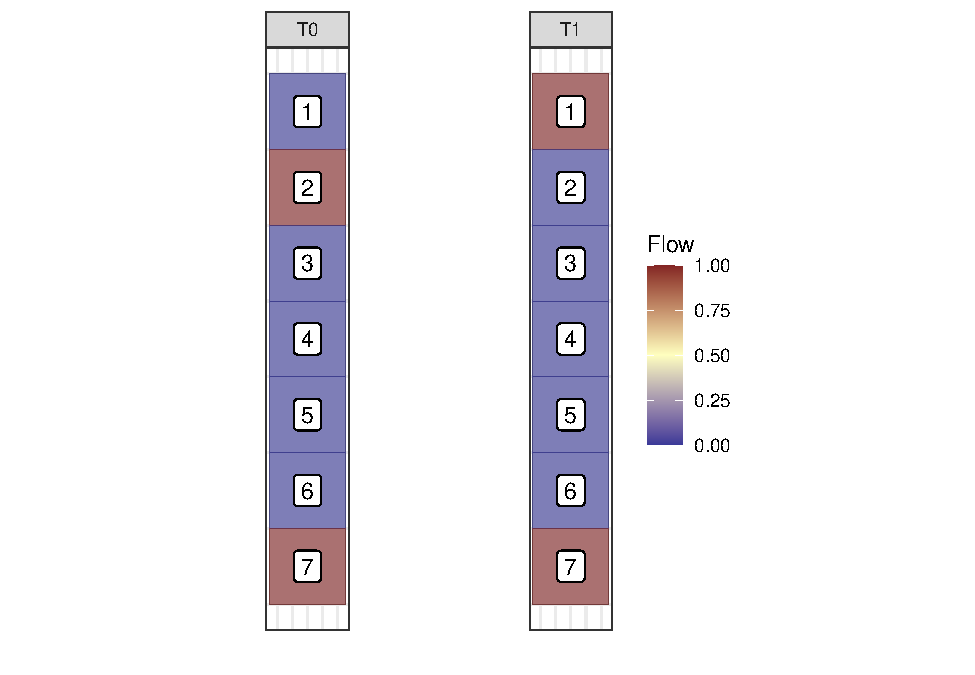
\includegraphics{TagetBasedNew_files/figure-latex/FinalStack-1.pdf}
\caption{\label{fig:FinalStack}Time-slice by time-slice prediction using Linear Cost Network Flow}
\end{figure}

\begin{figure}
\centering
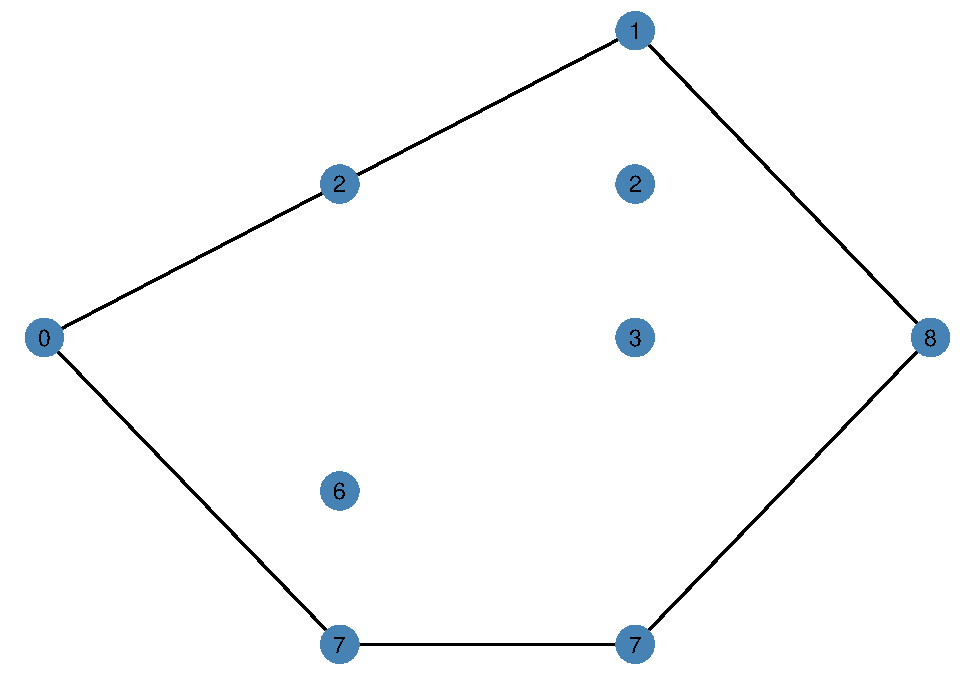
\includegraphics{TagetBasedNew_files/figure-latex/LinearGraphNEt-1.pdf}
\caption{\label{fig:LinearGraphNEt}Linear cost network flow solution shown as a graph}
\end{figure}

\begin{figure}
\centering
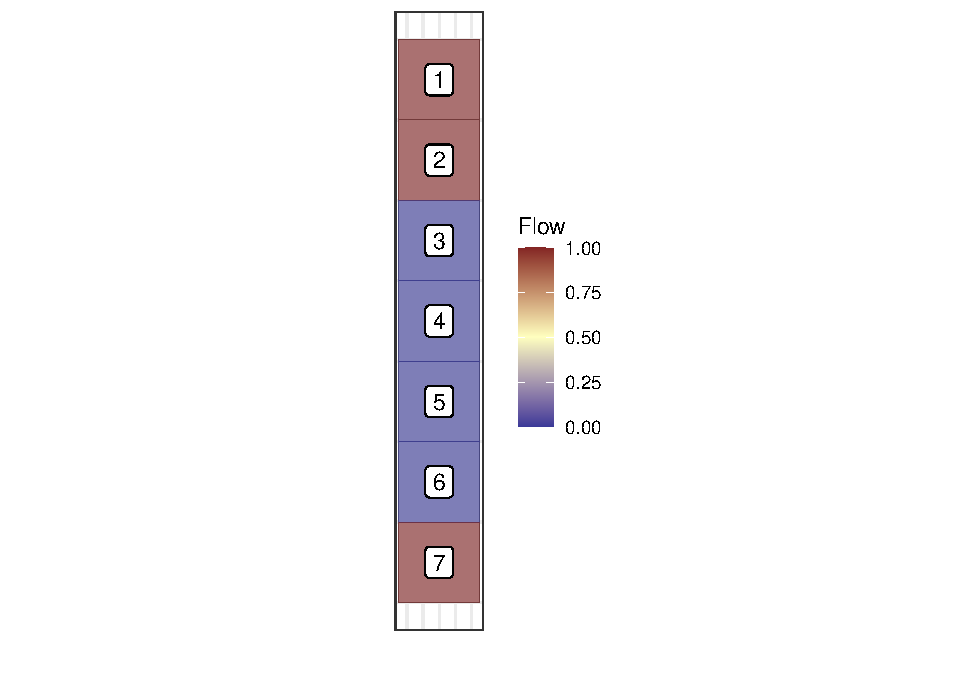
\includegraphics{TagetBasedNew_files/figure-latex/FinalSolution-1.pdf}
\caption{\label{fig:FinalSolution}Final solution using Linear Network Flow}
\end{figure}

\hypertarget{quadratic-solution}{%
\subsection{Quadratic Solution}\label{quadratic-solution}}

When we use quadratic cost network flow, what will happen is that when we decide on a number of chains to preserve, if there is only one choice for the flow to go through, the flow that will go through that node/edge is 1, but if there are more choices the flow will spread, and with it we will find out when there are more choices. When we solve the same problem shown above and we see the solution as seen in figure \ref{fig:FinalStackQuad} and, figure \ref{fig:QuadGraphNEt}, we see that in the upper half of the problem, the flow first goes only through cell 2 in \(T_1\), where the value of the flow is 1, but then when it goes to \(T_2\), that flow is spread evenly between the three posible cells that the flow could go to (cells 1, 2, and 3), with a value of 0.33. In the lower half of the problem we see that in \(T_1\) the flow goes from cells 6 and 7 where the flow is roughly 0.5 in each cell to cell 7 in \(T_2\) where the value of the flow is 1.

In each time-slice, there is one cell that is irreplaceble, in \(T_1\), there is no feaseable solution where cell 2 is not involved, and in \(T_2\) there are no feasable solutions where cell 7 is not involved. This is shown by the value of 1 in those cells for that time-slice as seen in figures \ref{fig:FinalStackQuad} and, \ref{fig:QuadGraphNEt}. To get the final value for the solution for each cell \(C_j\) (Irreplaceability index), we get the maximum value for each cell \(j\) amond all the different times \(i\) for time \(i\) to \(T\) as seen in equation \eqref{eq:Cell} and we get figure \ref{fig:FinalSolutionQuad}). This correctly identifies cells 2 and 7 as irrepleacable.

\begin{equation} 
  C_j = \max_{i = 0}^T{C_{j,i}}
  \label{eq:Cell}
\end{equation}

\begin{figure}
\centering
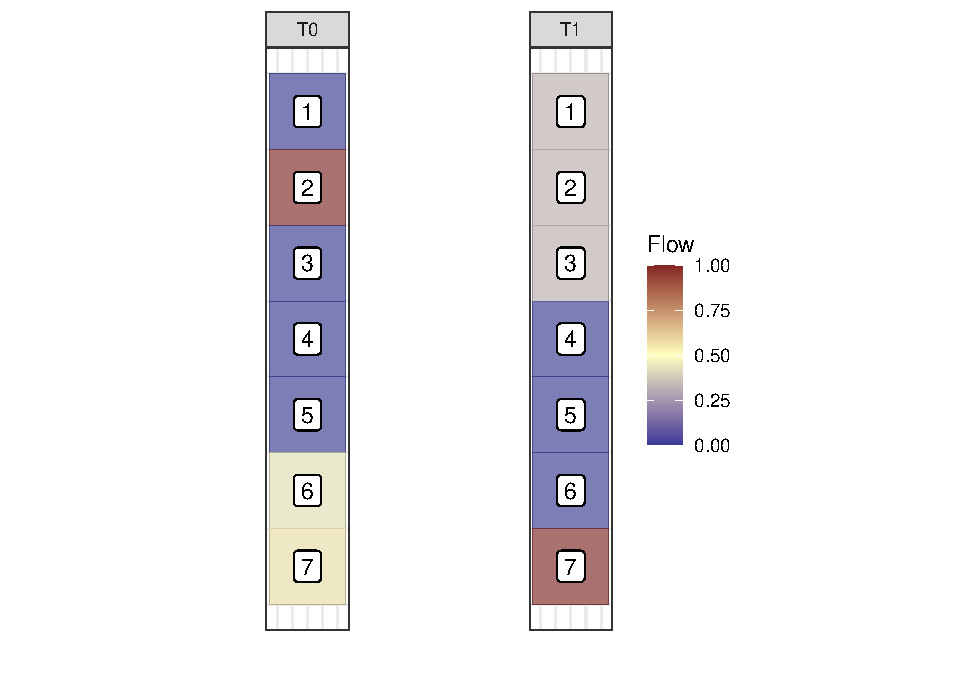
\includegraphics{TagetBasedNew_files/figure-latex/FinalStackQuad-1.pdf}
\caption{\label{fig:FinalStackQuad}Time-slice by time-slice prediction using the Quadratic Cost Network Flow}
\end{figure}

\begin{figure}
\centering
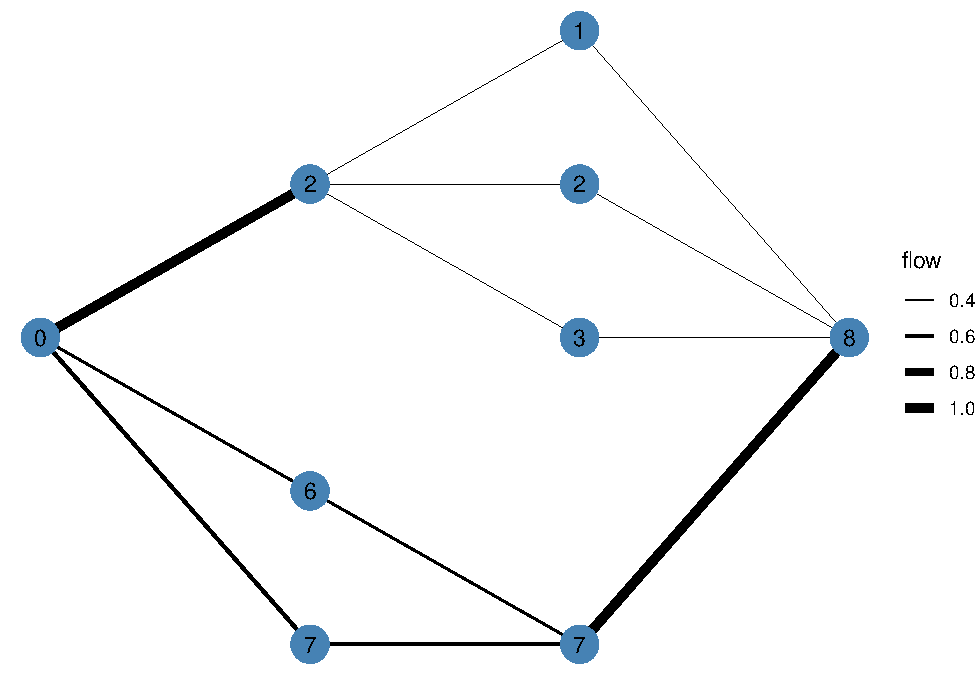
\includegraphics{TagetBasedNew_files/figure-latex/QuadGraphNEt-1.pdf}
\caption{\label{fig:QuadGraphNEt}Quadratic cost network flow solution shown as a graph}
\end{figure}

\begin{figure}
\centering
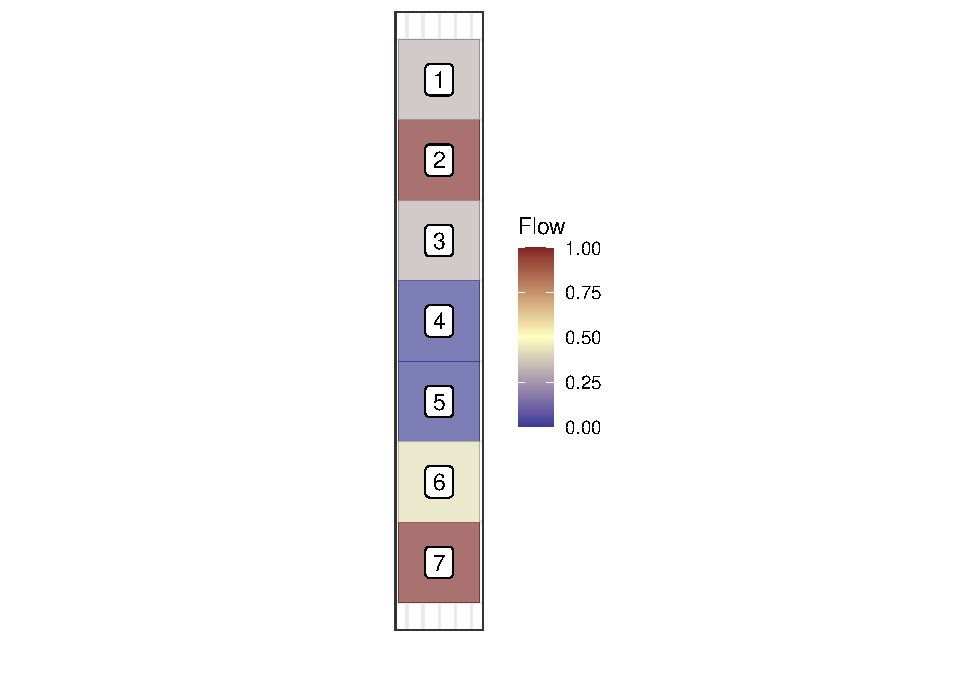
\includegraphics{TagetBasedNew_files/figure-latex/FinalSolutionQuad-1.pdf}
\caption{\label{fig:FinalSolutionQuad}Final solution using the quadratic cost algorithm}
\end{figure}

This solves the problem shown in the new linear algorithm for cells-IDs 1 through 3, where the solutions showed us only one of the possible solutions, and thus it gives us a buffer. As we see in figure \ref{fig:Sols}) the new linear algorithm gives us the most efficient solution, whereas the quadratic solution gives us the most resilient solution.

\begin{figure}
\centering
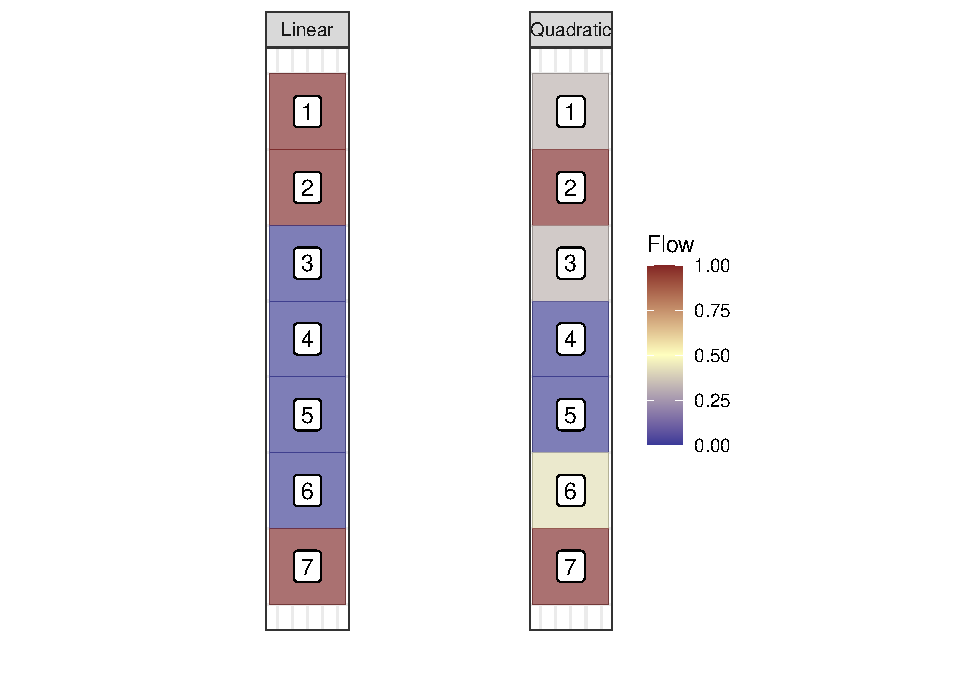
\includegraphics{TagetBasedNew_files/figure-latex/Sols-1.pdf}
\caption{\label{fig:Sols}All three solutions together}
\end{figure}

\hypertarget{results-for-the-quadratic-network-flow-algorithm-manuscript}{%
\subsection{Results for the Quadratic Network Flow algorithm manuscript}\label{results-for-the-quadratic-network-flow-algorithm-manuscript}}

The studied area was the Northern Tropical Andes, including the countries of Colombia, Venezuela and
Ecuador. To avoid pixels on countries' borders receiving a lower priority due to a boundary effect,
we extended the analyses to a buffer of 200 kilometers around their terrestrial domains. The study area
encompasses a total of 3,632,762 square kilometers. In that area we solved both linear and quadratic network flow to solve for the conservation of 671 species of Plants and Vertebrates. To combine the solution of every species, the Priority index \(P\) of every cell \(j\) (\(P_j\)) we used the squared sum of the root squared of the irreplaceability index value calculated for each cell \(C_j\) as calculated in equation \eqref{eq:Cell} for every species \(i\) in order to get a general solution for both algorithms using equation \eqref{eq:Priority}.

\begin{equation} 
  P_j = (\sum_{i=1}^{s}\sqrt{C_{j}})^2
  \label{eq:Priority}
\end{equation}

In figure \ref{fig:ComparisonSols}, we see the normalized solution for both algorithms, and we see that there seems to be almost no difference. However when we look at all the cells that take part in the solution (figure \ref{fig:Overlap}) we see that all the solutions in the linear network flow are contained within the quadratic network flow as expected. When we look at table \ref{tab:Pers}, we see that we need to use 16.6\% of the cells to get all the cells in the linear network flow solution, and only an extra 3.82\% of cells to add the buffer of the quadratic network flow.

\begin{figure}
\centering
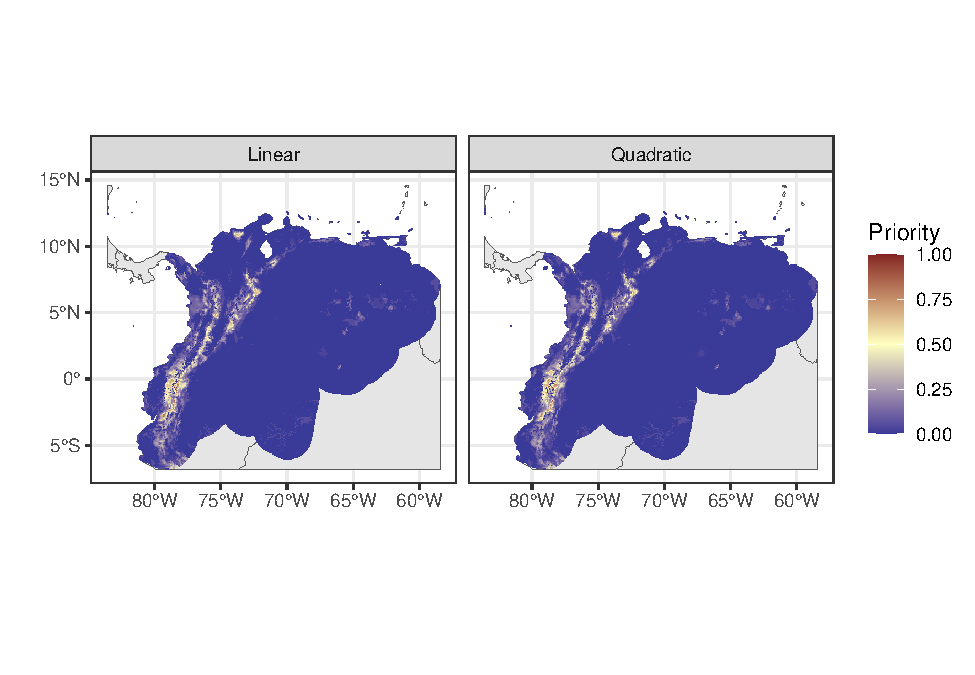
\includegraphics{TagetBasedNew_files/figure-latex/ComparisonSols-1.pdf}
\caption{\label{fig:ComparisonSols}Raw results of each of the algorithms}
\end{figure}

\begin{figure}
\centering
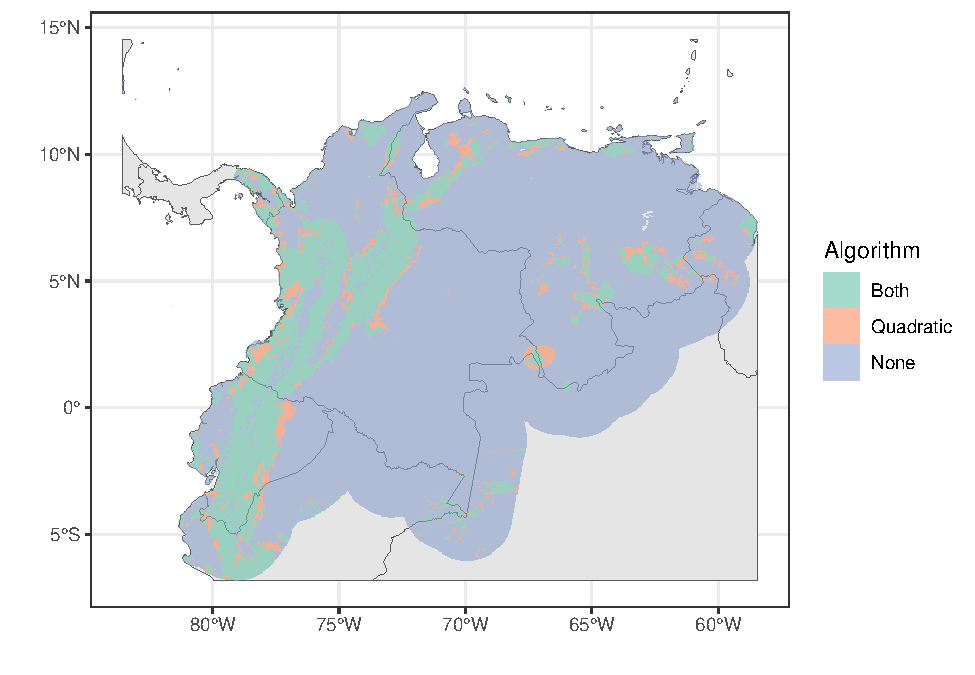
\includegraphics{TagetBasedNew_files/figure-latex/Overlap-1.pdf}
\caption{\label{fig:Overlap}This map shows the cells that are part of the solution in the Quadratic Cost Network Flow and in both algorithms. All the cells that are part of the Linear Cost Network Flow are also part of the solution of the Quadratic Cost Network Flow}
\end{figure}

\begin{table}[!h]

\caption{\label{tab:Pers}Number and percentage of cells that are part of the solution for both algorithms, for the quadratic solution only, and for no algorithm}
\centering
\begin{tabular}[t]{lrr}
\toprule
Algorithm & n & Percentage\\
\midrule
\rowcolor{gray!6}  Both & 25,083 & 16.60\\
Quadratic & 5,776 & 3.82\\
\rowcolor{gray!6}  None & 120,280 & 79.58\\
\bottomrule
\end{tabular}
\end{table}

\hypertarget{conclusions}{%
\section{Conclusions}\label{conclusions}}

There are several advantages in the use of Network Flow, since the results of each species is solved individually we can store them as an individual result using equation \eqref{eq:Cell}. This means that we could, for example, gain knowledge about a few of the 671 species in our example and instead of having to Run all the problem again, we can only run the models for the species for which we have new information and then add them together using equation \eqref{eq:Priority}. Also, we could do bootstrapping, jackknife or any other resampling techniques to get confidence intervals for our results giving us even more resilience.

At the same time since the optimization part of the problem is the one that is computing intensive it is quite easy and fast to test different version of equation \eqref{eq:Priority}, for example adding a Phylogenetic Rarity Index multiplier for each species to give more weight to phylogenetic groups that are less represented in the area.

If we look at the results in table \ref{tab:Pers} and figure \ref{fig:Overlap}, we can see that there is not much area added to the result of the Linear Cost Network Flow with just 3.82\% of cells added to the original solution. Furthermore, when we look at the prioritization index of both methods in Figure \ref{fig:ComparisonSols}, both seem almost indistinguishable, when we run a Spearman correlation between them, the Spearman's rank correlation rho between the prioritization values for the Quadratic and for the Linear Network Flow Algorithms is positive, significant and very large (rho = 0.92, S = 4.64e+13, p \textless{} .001). But we don't expect this to be true every time, there are at least four factors that will affect this, the dispersal distance selected for each species, the Range Size of the Species, if the species range is Contracting or Expanding, and the number of chains we want to preserve. The difference between the Linear and Quadratic Cost Network Flow are expected to be more different when the dipersal distance and ranges of the species is larger, when the range expands intead of retracts and if we choose less number of chains to preserve. The reason behind this is that all of this choices would diminish the number of irreplaceable cells, and thus divinding the flow through the network and generating more and more cells with any value other than zero that would be part of the buffer.

\hypertarget{references}{%
\section*{References}\label{references}}
\addcontentsline{toc}{section}{References}

\hypertarget{refs}{}
\leavevmode\hypertarget{ref-Ahuja93}{}%
Ahuja, Ravindra K., Thomas L. Magnanti, and James B. Orlin. 1993. \emph{Network Flows: Theory, Algorithms, and Applications}. Englewood Cliffs, NJ: Prentice Hall.

\leavevmode\hypertarget{ref-alagador2014shifting}{}%
Alagador, Diogo, Jorge Orestes Cerdeira, and Miguel Bastos Araújo. 2014. ``Shifting Protected Areas: Scheduling Spatial Priorities Under Climate Change.'' \emph{Journal of Applied Ecology} 51 (3). Wiley Online Library: 703--13.

\leavevmode\hypertarget{ref-araujo2004would}{}%
Araújo, Miguel B, Mar Cabeza, Wilfried Thuiller, Lee Hannah, and Paul H Williams. 2004. ``Would Climate Change Drive Species Out of Reserves? An Assessment of Existing Reserve-Selection Methods.'' \emph{Global Change Biology} 10 (9). Wiley Online Library: 1618--26.

\leavevmode\hypertarget{ref-beier2007linkage}{}%
Beier, P, DR Majka, and T Bayless. 2007. ``Linkage Designs for Arizona's Missing Linkages.'' \emph{Arizona Game and Fish Department, Phoenix}.

\leavevmode\hypertarget{ref-Boyle2019GNRS}{}%
Boyle, Brad. 2019. ``Geographic Name Resolution Service (Gnrs).'' \emph{GitHub Repository}. \url{https://github.com/ojalaquellueva/gnrs}; GitHub.

\leavevmode\hypertarget{ref-boyle2013taxonomic}{}%
Boyle, Brad, Nicole Hopkins, Zhenyuan Lu, Juan Antonio Raygoza Garay, Dmitry Mozzherin, Tony Rees, Naim Matasci, et al. 2013. ``The Taxonomic Name Resolution Service: An Online Tool for Automated Standardization of Plant Names.'' \emph{BMC Bioinformatics} 14 (1). BioMed Central: 16.

\leavevmode\hypertarget{ref-chen2011rapid}{}%
Chen, I-Ching, Jane K Hill, Ralf Ohlemüller, David B Roy, and Chris D Thomas. 2011. ``Rapid Range Shifts of Species Associated with High Levels of Climate Warming.'' \emph{Science} 333 (6045). American Association for the Advancement of Science: 1024--6.

\leavevmode\hypertarget{ref-cushman2013biological}{}%
Cushman, Samuel A, Brad McRae, Frank Adriaensen, Paul Beier, Mark Shirley, and Kathy Zeller. 2013. ``Biological Corridors and Connectivity {[}Chapter 21{]}.'' \emph{In: Macdonald, DW; Willis, KJ, Eds. Key Topics in Conservation Biology 2. Hoboken, NJ: Wiley-Blackwell. P. 384-404.} Wiley Online Library, 384--404.

\leavevmode\hypertarget{ref-de2018soilgrids}{}%
De Sousa, LM, GBM Heuvelink, NH Batjes, and B Kempen. 2018. ``SoilGrids: Using Big Data Solutions and Machine Learning Algorithms for Global Soil Mapping.'' In \emph{Scientific Symposium Fair Data Sciences for Green Life Sciences}, 1--1.

\leavevmode\hypertarget{ref-di2014quick}{}%
Di Minin, Enrico, Victoria Veach, Joona Lehtomäki, Federico Montesino Pouzols, Atte Moilanen, and others. 2014. ``A Quick Introduction to Zonation.'' Helsingin yliopisto.

\leavevmode\hypertarget{ref-fajardo_javier_2018_2669407}{}%
Fajardo, Javier, Derek Corcoran, Patrick R Roehrdanz, Lee Hannah, and Pablo A Marquet. 2020. ``GCM compareR: A Web Application to Assess Differences and Assist in the Selection of General Circulation Models for Climate Change Research.'' \emph{Methods in Ecology and Evolution}. Wiley Online Library.

\leavevmode\hypertarget{ref-fischer2009integrating}{}%
Fischer, Joern, Garry D Peterson, Toby A Gardner, Line J Gordon, Ioan Fazey, Thomas Elmqvist, Adam Felton, Carl Folke, and Stephen Dovers. 2009. ``Integrating Resilience Thinking and Optimisation for Conservation.'' \emph{Trends in Ecology \& Evolution} 24 (10). Elsevier: 549--54.

\leavevmode\hypertarget{ref-gregory2014forecasts}{}%
Gregory, Stephen D, Marc Ancrenaz, Barry W Brook, Benoit Goossens, Raymond Alfred, Laurentius N Ambu, and Damien A Fordham. 2014. ``Forecasts of Habitat Suitability Improve Habitat Corridor Efficacy in Rapidly Changing Environments.'' \emph{Diversity and Distributions} 20 (9). Wiley Online Library: 1044--57.

\leavevmode\hypertarget{ref-hannah2007protected}{}%
Hannah, Lee, Guy Midgley, Sandy Andelman, Miguel Araújo, Greg Hughes, Enrique Martinez-Meyer, Richard Pearson, and Paul Williams. 2007. ``Protected Area Needs in a Changing Climate.'' \emph{Frontiers in Ecology and the Environment} 5 (3). Wiley Online Library: 131--38.

\leavevmode\hypertarget{ref-Hanson2019}{}%
Hanson, Jeffrey O, Richard Schuster, Nina Morrell, Matthew Strimas-Mackey, Matthew E Watts, Peter Arcese, Joseph Bennett, and Hugh P Possingham. 2019. \emph{Prioritizr: Systematic Conservation Prioritization in R}. \url{https://CRAN.R-project.org/package=prioritizr}.

\leavevmode\hypertarget{ref-Hijmans_Dismo}{}%
Hijmans, Robert J., Steven Phillips, John Leathwick, and Jane Elith. 2017. \emph{Dismo: Species Distribution Modeling}. \url{https://CRAN.R-project.org/package=dismo}.

\leavevmode\hypertarget{ref-jenkins2015us}{}%
Jenkins, Clinton N, Kyle S Van Houtan, Stuart L Pimm, and Joseph O Sexton. 2015. ``US Protected Lands Mismatch Biodiversity Priorities.'' \emph{Proceedings of the National Academy of Sciences} 112 (16). National Acad Sciences: 5081--6.

\leavevmode\hypertarget{ref-jones2016incorporating}{}%
Jones, Kendall R, James EM Watson, Hugh P Possingham, and Carissa J Klein. 2016. ``Incorporating Climate Change into Spatial Conservation Prioritisation: A Review.'' \emph{Biological Conservation} 194. Elsevier: 121--30.

\leavevmode\hypertarget{ref-lawler2013projected}{}%
Lawler, JJ, AS Ruesch, JD Olden, and BH McRae. 2013. ``Projected Climate-Driven Faunal Movement Routes.'' \emph{Ecology Letters} 16 (8). Wiley Online Library: 1014--22.

\leavevmode\hypertarget{ref-lenoir2008significant}{}%
Lenoir, Jonathan, Jean-Claude Gégout, PA Marquet, P De Ruffray, and H Brisse. 2008. ``A Significant Upward Shift in Plant Species Optimum Elevation During the 20th Century.'' \emph{Science} 320 (5884). American Association for the Advancement of Science: 1768--71.

\leavevmode\hypertarget{ref-marquet_2019}{}%
Marquet, Pablo, Janeth Lessman, and Rebecca Shaw. 2019. ``Protected-Area Management and Climate Change.'' In \emph{Biodiversity and Climate Change: Transforming the Biosphere}, edited by Thomas E Lovejoy, Lee Hannah, and Edward O Wilson, 283--93. New Haven, Connecticut: Yale University Press.

\leavevmode\hypertarget{ref-merow2014we}{}%
Merow, Cory, Mathew J Smith, Thomas C Edwards Jr, Antoine Guisan, Sean M McMahon, Signe Normand, Wilfried Thuiller, Rafael O Wüest, Niklaus E Zimmermann, and Jane Elith. 2014. ``What Do We Gain from Simplicity Versus Complexity in Species Distribution Models?'' \emph{Ecography} 37 (12). Wiley Online Library: 1267--81.

\leavevmode\hypertarget{ref-merow2013practical}{}%
Merow, Cory, Matthew J Smith, and John A Silander Jr. 2013. ``A Practical Guide to Maxent for Modeling Species' Distributions: What It Does, and Why Inputs and Settings Matter.'' \emph{Ecography} 36 (10). Wiley Online Library: 1058--69.

\leavevmode\hypertarget{ref-naidoo2007global}{}%
Naidoo, Robin, and Takuya Iwamura. 2007. ``Global-Scale Mapping of Economic Benefits from Agricultural Lands: Implications for Conservation Priorities.'' \emph{Biological Conservation} 140 (1-2). Elsevier: 40--49.

\leavevmode\hypertarget{ref-nunez2013connectivity}{}%
Nuñez, Tristan A, Joshua J Lawler, Brad H McRae, D John Pierce, Meade B Krosby, Darren M Kavanagh, Peter H Singleton, and Joshua J Tewksbury. 2013. ``Connectivity Planning to Address Climate Change.'' \emph{Conservation Biology} 27 (2). Wiley Online Library: 407--16.

\leavevmode\hypertarget{ref-phillips2006maximum}{}%
Phillips, Steven J, Robert P Anderson, and Robert E Schapire. 2006. ``Maximum Entropy Modeling of Species Geographic Distributions.'' \emph{Ecological Modelling} 190 (3-4). Elsevier: 231--59.

\leavevmode\hypertarget{ref-phillips2008optimizing}{}%
Phillips, Steven J, Paul Williams, Guy Midgley, and Aaron Archer. 2008. ``Optimizing Dispersal Corridors for the Cape Proteaceae Using Network Flow.'' \emph{Ecological Applications} 18 (5). Wiley Online Library: 1200--1211.

\leavevmode\hypertarget{ref-regos2016predicting}{}%
Regos, Adrián, Manuela D'Amen, Nicolas Titeux, Sergi Herrando, Antoine Guisan, and Lluı's Brotons. 2016. ``Predicting the Future Effectiveness of Protected Areas for Bird Conservation in Mediterranean Ecosystems Under Climate Change and Novel Fire Regime Scenarios.'' \emph{Diversity and Distributions} 22 (1). Wiley Online Library: 83--96.

\leavevmode\hypertarget{ref-reside2017trade}{}%
Reside, April Elizabeth, Jeremy VanDerWal, and Catherine Moran. 2017. ``Trade-Offs in Carbon Storage and Biodiversity Conservation Under Climate Change Reveal Risk to Endemic Species.'' \emph{Biological Conservation} 207. Elsevier: 9--16.

\leavevmode\hypertarget{ref-rodrigues2004effectiveness}{}%
Rodrigues, Ana SL, Sandy J Andelman, Mohamed I Bakarr, Luigi Boitani, Thomas M Brooks, Richard M Cowling, Lincoln DC Fishpool, et al. 2004. ``Effectiveness of the Global Protected Area Network in Representing Species Diversity.'' \emph{Nature} 428 (6983). Nature Publishing Group: 640.

\leavevmode\hypertarget{ref-rosenberg1997biological}{}%
Rosenberg, Daniel K, Barry R Noon, and E Charles Meslow. 1997. ``Biological Corridors: Form, Function, and Efficacy.'' \emph{BioScience} 47 (10). JSTOR: 677--87.

\leavevmode\hypertarget{ref-tuanmu2014global}{}%
Tuanmu, Mao-Ning, and Walter Jetz. 2014. ``A Global 1-Km Consensus Land-Cover Product for Biodiversity and Ecosystem Modelling.'' \emph{Global Ecology and Biogeography} 23 (9). Wiley Online Library: 1031--45.

\leavevmode\hypertarget{ref-unep2018ngs}{}%
UNEP-WCMC, IUCN. 2018. ``NGS (2018).'' \emph{Protected Planet Report}.

\leavevmode\hypertarget{ref-williams2005planning}{}%
Williams, Paul, Lee Hannah, Sandy Andelman, Guy Midgley, Miguel Araújo, Greg Hughes, Lisa Manne, Enrique Martinez-Meyer, and Richard Pearson. 2005. ``Planning for Climate Change: Identifying Minimum-Dispersal Corridors for the Cape Proteaceae.'' \emph{Conservation Biology} 19 (4). Wiley Online Library: 1063--74.

\leavevmode\hypertarget{ref-zappa2017storylines}{}%
Zappa, Giuseppe, and Theodore G Shepherd. 2017. ``Storylines of Atmospheric Circulation Change for European Regional Climate Impact Assessment.'' \emph{Journal of Climate} 30 (16): 6561--77.

\end{document}
